% Stochastic Modeling and Simulation of Vehicle Headways on Highways -- condensed version
% Build: pdflatex main && bibtex main && pdflatex main && pdflatex main
% Numbers come from results.tex and tables/*.tex (generated from outputs/ by headway.make_report_assets and condense_tables.py).
\documentclass[10pt,a4paper]{article}

\usepackage[T1]{fontenc}
\usepackage[utf8]{inputenc}
\usepackage{lmodern}
\usepackage[a4paper,top=2.3cm,bottom=2.3cm,left=2.3cm,right=2.3cm]{geometry}
\usepackage{amsmath,amssymb}
\usepackage{textcomp}
\usepackage{graphicx}
\usepackage{booktabs,array,tabularx}
\usepackage{float}
\usepackage{enumitem}
\usepackage{listings}
\usepackage{xcolor}
\usepackage{microtype}
\usepackage{xurl}
\usepackage{needspace}
\usepackage[font=small,labelfont=bf,skip=4pt]{caption}
\usepackage[numbers,sort&compress]{natbib}
\usepackage[colorlinks=true,linkcolor=blue!50!black,citecolor=blue!50!black,urlcolor=blue!50!black]{hyperref}
\setlength{\emergencystretch}{3em}
\setlist{itemsep=1pt,topsep=2pt,parsep=0pt}
\setlength{\parskip}{2pt}
\renewcommand{\arraystretch}{1.08}
\setlength{\textfloatsep}{8pt plus 2pt minus 2pt}
\setlength{\floatsep}{7pt plus 2pt minus 2pt}
\setlength{\intextsep}{7pt plus 2pt minus 2pt}
\setlength{\bibsep}{1pt}
\renewcommand{\bibfont}{\small}
\newcolumntype{Y}{>{\raggedright\arraybackslash}X}
\lstset{language=Python,basicstyle=\ttfamily\scriptsize,breaklines=true,frame=tb,numbers=left,
        numberstyle=\tiny\color{gray},keywordstyle=\bfseries,commentstyle=\itshape\color{gray},
        showstringspaces=false,xleftmargin=1.5em,captionpos=b,belowskip=0.6em,aboveskip=0.6em}
\numberwithin{equation}{section}

\newcommand{\E}{\mathbb{E}}
\newcommand{\Var}{\operatorname{Var}}
\newcommand{\Prob}{\mathbb{P}}
\newcommand{\Wvec}{W_{\mathrm{vec}}}
\newcommand{\Wtime}{W_{\mathrm{time}}}
% GENERATED by `python -m headway.make_report_assets` from outputs/*/*.csv -- do not edit by hand.
\newcommand{\hdN}{1{,}225{,}460}
\newcommand{\hdRuns}{112{,}841}
\newcommand{\hdTrans}{1{,}112{,}619}
\newcommand{\hdMean}{2.21}
\newcommand{\hdMedian}{1.66}
\newcommand{\hdStd}{1.73}
\newcommand{\hdMin}{0.50}
\newcommand{\hdMax}{24.96}
\newcommand{\hdA}{0.954}
\newcommand{\hdB}{0.540}
\newcommand{\hdKappa}{0.617}
\newcommand{\hdALo}{0.950}
\newcommand{\hdAHi}{0.959}
\newcommand{\hdBLo}{0.539}
\newcommand{\hdBHi}{0.540}
\newcommand{\hdKLProp}{0.0036}
\newcommand{\hdKLPropPaper}{0.0036}
\newcommand{\hdKLSLN}{0.0026}
\newcommand{\hdKLBurr}{0.0043}
\newcommand{\hdKLLLog}{0.0092}
\newcommand{\hdKLBest}{Shifted Log-normal}
\newcommand{\hdKLBestPaper}{Proposed}
\newcommand{\hdKLRankProp}{2}
\newcommand{\hdKLRankPropPaper}{1}
\newcommand{\hdKLMaxDiffPaper}{0.0058}
\newcommand{\hdKLMaxDiffPaperName}{Log-logistic}
\newcommand{\hdKLMaxDiffTrunc}{0.0455}
\newcommand{\hdKLMaxDiffTruncName}{Weibull}
\newcommand{\hdWvecBest}{Shifted Log-normal}
\newcommand{\hdWvecBestPaper}{Proposed}
\newcommand{\hdWvecMaxDiffPaper}{0.0006}
\newcommand{\hdWvecMaxDiffPaperName}{Weibull}
\newcommand{\hdWtimeBest}{Shifted Log-normal}
\newcommand{\hdWtimeBestVal}{0.048}
\newcommand{\hdWtimeProp}{0.072}
\newcommand{\hdRhatMaxTrunc}{1.004}
\newcommand{\hdRhatMaxPaper}{1.005}
\newcommand{\hdRhatMaxPaperName}{Shifted Exponential}
\newcommand{\hdAccMin}{21.0}
\newcommand{\hdAccMax}{25.6}
\newcommand{\hdEssMin}{609}
\newcommand{\hdMcmcTime}{14.5}
\newcommand{\hdRate}{0.4520}
\newcommand{\hdFlow}{1{,}627}
\newcommand{\hdCV}{0.61}
\newcommand{\hdCVInv}{1.6}
\newcommand{\hdRenMeanMax}{0.2}
\newcommand{\hdRenVarMax}{3.8}
\newcommand{\hdRenVarMaxT}{300}
\newcommand{\hdKsNormal}{0.022}
\newcommand{\hdKsPoisson}{0.071}
\newcommand{\hdPiC}{0.454}
\newcommand{\hdRecC}{2.20}
\newcommand{\hdPiP}{0.435}
\newcommand{\hdRecP}{2.30}
\newcommand{\hdPiF}{0.111}
\newcommand{\hdRecF}{9.03}
\newcommand{\hdSojC}{33.7}
\newcommand{\hdSojP}{25.8}
\newcommand{\hdSojF}{19.3}
\newcommand{\hdMixTVTwenty}{0.182}
\newcommand{\hdMixTVSixty}{0.022}
\newcommand{\hdRunLen}{10.9}
\newcommand{\hdLagOne}{0.906}
\newcommand{\hdLagFive}{0.601}
\newcommand{\hdBand}{0.0019}
\newcommand{\hdCKtwo}{0.006}
\newcommand{\hdCKfive}{0.055}
\newcommand{\hdStatTV}{0.014}
\newcommand{\hdSecondTV}{0.0014}
\newcommand{\hdSecondGsq}{1046.4}
\newcommand{\hdShExpLambda}{0.585}
\newcommand{\hdShExpGammaPaper}{0.500}
\newcommand{\hdShExpLambdaPaper}{0.585}
\newcommand{\hdShExpKLTrunc}{0.0080}
\newcommand{\hdShExpKLPaper}{0.0080}
\newcommand{\hdProposedMean}{2.22}
\newcommand{\hdProposedStd}{1.64}
\newcommand{\hdBurrAlpha}{1.464}
\newcommand{\ngN}{117{,}068}
\newcommand{\ngRuns}{3{,}207}
\newcommand{\ngTrans}{113{,}861}
\newcommand{\ngMean}{3.08}
\newcommand{\ngMedian}{2.56}
\newcommand{\ngStd}{2.08}
\newcommand{\ngMin}{0.50}
\newcommand{\ngMax}{24.98}
\newcommand{\ngA}{2.336}
\newcommand{\ngB}{0.524}
\newcommand{\ngKappa}{0.646}
\newcommand{\ngALo}{2.326}
\newcommand{\ngAHi}{2.345}
\newcommand{\ngBLo}{0.522}
\newcommand{\ngBHi}{0.527}
\newcommand{\ngKLProp}{0.0760}
\newcommand{\ngKLPropPaper}{0.0760}
\newcommand{\ngKLSLN}{0.0153}
\newcommand{\ngKLBurr}{0.0015}
\newcommand{\ngKLLLog}{0.0167}
\newcommand{\ngKLBest}{Burr}
\newcommand{\ngKLBestPaper}{Burr}
\newcommand{\ngKLRankProp}{4}
\newcommand{\ngKLRankPropPaper}{4}
\newcommand{\ngKLMaxDiffPaper}{0.0311}
\newcommand{\ngKLMaxDiffPaperName}{Shifted Exponential}
\newcommand{\ngKLMaxDiffTrunc}{0.0311}
\newcommand{\ngKLMaxDiffTruncName}{Shifted Exponential}
\newcommand{\ngWvecBest}{Burr}
\newcommand{\ngWvecBestPaper}{Burr}
\newcommand{\ngWvecMaxDiffPaper}{0.0110}
\newcommand{\ngWvecMaxDiffPaperName}{Gamma}
\newcommand{\ngWtimeBest}{Burr}
\newcommand{\ngWtimeBestVal}{0.031}
\newcommand{\ngWtimeProp}{0.225}
\newcommand{\ngRhatMaxTrunc}{1.005}
\newcommand{\ngRhatMaxPaper}{1.006}
\newcommand{\ngRhatMaxPaperName}{Burr}
\newcommand{\ngAccMin}{19.1}
\newcommand{\ngAccMax}{26.5}
\newcommand{\ngEssMin}{437}
\newcommand{\ngMcmcTime}{16.3}
\newcommand{\ngRate}{0.3242}
\newcommand{\ngFlow}{1{,}167}
\newcommand{\ngCV}{0.46}
\newcommand{\ngCVInv}{2.2}
\newcommand{\ngRenMeanMax}{0.2}
\newcommand{\ngRenVarMax}{7.0}
\newcommand{\ngRenVarMaxT}{30}
\newcommand{\ngKsNormal}{0.038}
\newcommand{\ngKsPoisson}{0.127}
\newcommand{\ngPiC}{0.096}
\newcommand{\ngRecC}{10.42}
\newcommand{\ngPiP}{0.730}
\newcommand{\ngRecP}{1.37}
\newcommand{\ngPiF}{0.174}
\newcommand{\ngRecF}{5.75}
\newcommand{\ngSojC}{3.9}
\newcommand{\ngSojP}{12.5}
\newcommand{\ngSojF}{4.9}
\newcommand{\ngMixTVTwenty}{0.003}
\newcommand{\ngMixTVSixty}{0.000}
\newcommand{\ngRunLen}{36.5}
\newcommand{\ngLagOne}{0.727}
\newcommand{\ngLagFive}{0.426}
\newcommand{\ngBand}{0.0058}
\newcommand{\ngCKtwo}{0.092}
\newcommand{\ngCKfive}{0.226}
\newcommand{\ngStatTV}{0.008}
\newcommand{\ngSecondTV}{0.0400}
\newcommand{\ngSecondGsq}{4291.5}
\newcommand{\ngShExpLambda}{0.387}
\newcommand{\ngShExpGammaPaper}{0.500}
\newcommand{\ngShExpLambdaPaper}{0.387}
\newcommand{\ngShExpKLTrunc}{0.2713}
\newcommand{\ngShExpKLPaper}{0.2713}
\newcommand{\ngProposedMean}{2.95}
\newcommand{\ngProposedStd}{1.68}
\newcommand{\ngBurrAlpha}{4.916}
\newcommand{\ngPeriodTwoN}{292{,}831}
\newcommand{\ngPeriodTwoMean}{4.04}
\newcommand{\ngBothN}{409{,}899}
\newcommand{\ngBothMean}{3.77}
\newcommand{\ngImpliedLo}{2.77}
\newcommand{\ngImpliedHi}{3.04}
\newcommand{\ngImpliedN}{5}
\newcommand{\hdSLNGamma}{\textminus{}0.001}
\newcommand{\ngSLNGamma}{0.500}
\newcommand{\hdDetN}{108{,}842}
\newcommand{\hdDetUnits}{337}
\newcommand{\hdDetMean}{3.08}
\newcommand{\hdDetMedian}{2.11}
\newcommand{\hdDetCV}{1.18}
\newcommand{\hdDetFlow}{1{,}168}
\newcommand{\hdDetFracBelow}{0.4}
\newcommand{\hdDetFracAbove}{0.2}
\newcommand{\hdDetLagOne}{0.031}
\newcommand{\hdDetLagTwo}{\textminus{}0.009}
\newcommand{\hdDetBand}{0.0060}
\newcommand{\hdDetKsD}{0.172}
\newcommand{\hdDetFanoObs}{0.96}
\newcommand{\hdDetFanoRen}{0.77}
\newcommand{\hdDetWindows}{5{,}383}
\newcommand{\hdDetSeries}{334}
\newcommand{\hdDetMeanCount}{19.5}
\newcommand{\ngDetN}{2{,}046}
\newcommand{\ngDetUnits}{6}
\newcommand{\ngDetMean}{2.64}
\newcommand{\ngDetMedian}{2.30}
\newcommand{\ngDetCV}{0.30}
\newcommand{\ngDetFlow}{1{,}364}
\newcommand{\ngDetFracBelow}{0.3}
\newcommand{\ngDetFracAbove}{0.0}
\newcommand{\ngDetLagOne}{0.125}
\newcommand{\ngDetLagTwo}{0.091}
\newcommand{\ngDetBand}{0.0434}
\newcommand{\ngDetKsD}{0.324}
\newcommand{\ngDetFanoObs}{0.52}
\newcommand{\ngDetFanoRen}{0.29}
\newcommand{\ngDetWindows}{86}
\newcommand{\ngDetSeries}{6}
\newcommand{\ngDetMeanCount}{22.6}
\newcommand{\nTests}{52}


\title{\vspace{-1.2cm}\textbf{Stochastic Modeling and Simulation of Vehicle Headways on Highways:\\
A Bayesian Headway Distribution, Renewal Arrival Process, and Regime Markov Chain\\
Using highD and NGSIM Trajectory Datasets}}
\author{%
\begin{tabular}[t]{@{}ccc@{}}
\textbf{Sanidhya Joshi} & \textbf{Kaustabh Kadam} & \textbf{Dev Dharsandiya}\\
(Team Leader) & & \\
Roll No.\ S20240010214 & Roll No.\ S20240010114 & Roll No.\ S20240010058
\end{tabular}\\[1.2ex]
International Institute of Information Technology, Sri City, India}
\date{}

\begin{document}
\maketitle
\vspace{-1.2em}

%================================================================================================
\begin{abstract}
\noindent Vehicle time headways govern lane capacity, safety margins and the variability of arrival counts, yet no single standard distribution fits all traffic conditions.
This paper treats headways from two public trajectory datasets, highD (\hdN{} one-second headways) and NGSIM I-80 (\ngN{}), as a stochastic system.
A recently proposed two-parameter density, $f(t\mid a,b)\propto b^{|t-a|}$, is compared with six standard distributions by Bayesian estimation with a Metropolis--Hastings sampler;
arrivals are modelled by a headway-driven renewal counting process and car-following regimes by a three-state Markov chain estimated from within-trajectory transitions.
With the published likelihood the proposed distribution has the lowest Kullback--Leibler divergence on highD (\hdKLPropPaper) and ranks fourth on NGSIM, as published; conditioning the likelihood on the $[0.5,25]$~s observation window makes the shifted log-normal best on highD (\hdKLSLN).
All 28 posteriors converge (split $\hat R\le\ngRhatMaxPaper$). Simulated renewal counts match renewal theory and are more regular than Poisson (variance-to-mean ratios \hdCV{} and \ngCV), but detector inter-arrival times reconstructed from the trajectories
show that one-minute highD counts are nearly Poisson (\hdDetFanoObs), and one-second headway sequences are strongly autocorrelated (lag-1 \hdLagOne).
\end{abstract}
\noindent\textbf{Keywords:} traffic headway; Bayesian inference; Metropolis--Hastings; renewal process; Markov chain; highD; NGSIM.

%================================================================================================
\section{Introduction}\label{sec:intro}
The time headway between a vehicle and its leader in the same lane is a basic microscopic variable of traffic flow. The reciprocal of its mean is the flow a lane carries in car-following conditions,
its lower tail governs rear-end risk, and its distribution drives capacity analysis, signal timing and microscopic simulation. Headways depend on driver, vehicle type, speed and volume, and the literature
has proposed many distributions without converging on one~\cite{leungbootnak}.
Leungbootnak et al.~\cite{leungbootnak} proposed a two-parameter density, $f(t\mid a,b)\propto b^{|t-a|}$, and compared it with six standard distributions on five trajectory datasets.
This project reproduces that comparison on two of them, highD and NGSIM, and places the fitted headway model inside two stochastic processes (a renewal counting process for vehicle arrivals and a Markov chain for car-following regimes), each verified against theory, simulation and data.

\noindent\textbf{Objectives.} (i)~Estimate seven headway distributions on highD and NGSIM by Bayesian MCMC and compare their fit; (ii)~reproduce the published results and identify where they differ and why;
(iii)~build a renewal counting process from the headways and compare it with renewal theory, Poisson arrivals and detector counts reconstructed from the trajectories;
(iv)~build a three-regime Markov chain from within-trajectory transitions and test its assumptions.

\noindent\textbf{Contributions.} (i)~A reproduction of the headway comparison of~\cite{leungbootnak}, with the sample and metric definitions needed to reproduce it.
(ii)~A statistical audit: the published likelihood ignores the truncation of the data to $[0.5,25]$~s, and conditioning on it changes the highD ranking (Section~\ref{sec:real});
a non-converging posterior (shifted exponential, highD) is traced to its likelihood geometry and removed (Section~\ref{sec:conv}); the Wasserstein distance of the published study admits two non-equivalent readings (Section~\ref{sec:math}).
(iii)~Renewal and Markov models built on these headways, with their assumptions tested on real within-trajectory sequences.
(iv)~A reconstruction of detector inter-arrival times that separates what the headway-driven renewal model predicts from what a detector counts (Section~\ref{sec:detmethod}).
Section~\ref{sec:data} describes the data, Section~\ref{sec:math} the mathematical models, Section~\ref{sec:method} the methodology and implementation, Section~\ref{sec:results} the results, and Sections~\ref{sec:limits}--\ref{sec:conclusion} the limitations and conclusions.

%================================================================================================
\section{Literature Review}\label{sec:lit}
\textbf{Classical headway distributions.} Adams~\cite{adams1936} described the intervals between vehicles passing a point by the negative exponential law, equivalent to a Poisson count of vehicles.
Its density is largest at zero headway, which real following drivers cannot produce, which motivated shifted and composite forms. Cowan~\cite{cowan1975} distinguished \emph{tracking} headways (a vehicle following its leader) from \emph{free} headways and mixed the two in
composite models. The shifted exponential, log-normal, Weibull, gamma, log-logistic and Burr families recur in the literature reviewed in~\cite{leungbootnak}; each describes a single regime, so the best-fitting family changes with traffic conditions.

\textbf{Bayesian headway modelling.} Bayesian estimation by MCMC quantifies parameter uncertainty and fits all candidates in one framework. Leungbootnak et al.~\cite{leungbootnak} estimate their proposed density and six baselines by Metropolis--Hastings~\cite{hastings1970} on five datasets,
and Wu et al.~\cite{wu2023} average several headway distributions by Bayesian model averaging because no single one wins everywhere.

\textbf{Renewal processes in traffic.} A renewal process has i.i.d.\ inter-event times~\cite{cox1962,ross1996}; taking headways as inter-arrival times gives a model of the vehicle count at a point, with the Poisson process as the exponential special case.
A non-exponential headway law allows arrivals more regular than Poisson, but the independence assumption must be tested.

\textbf{Markov chains in traffic.} A finite Markov chain~\cite{norris1997} describes movement between regimes with probabilities that depend on the current state;
Chen et al.~\cite{chen2010} developed a Markov model of the headway and spacing distribution. Its stationary distribution, recurrence times and persistence summarise regime dynamics.

\textbf{Gap.} The reproduced study~\cite{leungbootnak} compares distributions but does not embed them in a stochastic process, test the independence of successive headways, or report arrival-count and regime dynamics;
it also leaves the treatment of truncation in the likelihood, the Wasserstein definition and the NGSIM sample open. This paper addresses these points and checks how far a headway-driven renewal model describes what a detector actually counts.

%================================================================================================
\section{Dataset Description and Preprocessing}\label{sec:data}
\textbf{highD}~\cite{krajewski2018} contains drone-recorded trajectories on German highways (60 recordings, 25~Hz; position, velocity, lane, \texttt{precedingId} and the time headway \texttt{thw}); it describes uninterrupted human-driven flow.
\textbf{NGSIM}~\cite{ngsim} is the FHWA trajectory dataset; we use the I-80 data (10~Hz; vehicle, frame, lane, \texttt{Preceding}, \texttt{Time\_Headway}, \texttt{Local\_Y}, \texttt{Global\_Time}).
The published study used the reconstructed I-80 trajectories, whereas the data used here is the original Data.gov export.

\textbf{Sampling and filtering.} Following~\cite{leungbootnak}: (1)~one sample per second per follower (every 25th frame in highD, every 10th in NGSIM); (2)~only records with a preceding vehicle in the same lane;
(3)~headways below $\alpha=0.5$~s (below the minimum safe headway) or above $T=25$~s (not car following) are discarded; no other outlier rule is applied.
The headway is the dataset's own time-headway field: the gap between a follower and its leader at one instant, \emph{not} the time between successive vehicles crossing a fixed point (the \emph{detector inter-arrival time}, Section~\ref{sec:detmethod}).
Retained headways are ordered by vehicle and time, and every stretch of consecutive seconds of one vehicle is labelled a \emph{trajectory run}; Markov transitions and autocorrelations are counted only within runs.

\textbf{NGSIM period.} The export contains two recording periods. The first gives \ngN{} headways (mean \ngMean~s), the second \ngPeriodTwoN{} (mean \ngPeriodTwoMean~s). The published study does not say which it used; the mean headways implied by its fitted NGSIM parameters
(\ngImpliedLo--\ngImpliedHi~s for \ngImpliedN{} distributions) are close to the first period, which we therefore use. This is an inference, and the published NGSIM sample is not exactly reproduced.

\begin{table}[!tb]
\centering\small
\caption{Datasets and retained one-second headway samples (headways in seconds; Std: standard deviation). A run is a stretch of consecutive one-second samples of one follower.}
\label{tab:data}
\begin{tabularx}{\textwidth}{@{}lYY@{}}
\toprule
 & highD & NGSIM (I-80) \\
\midrule
Provider; region; sensor & RWTH Aachen; German highways; drone & FHWA; California; video cameras \\
Frame rate; selection used & 25~Hz; all 60 recordings & 10~Hz; first recording period \\
Retained headways & \hdN & \ngN \\
Mean / median / Std (s) & \hdMean\ / \hdMedian\ / \hdStd & \ngMean\ / \ngMedian\ / \ngStd \\
Min / max (s) & \hdMin\ / \hdMax & \ngMin\ / \ngMax \\
Runs; mean run length (s) & \hdRuns; \hdRunLen & \ngRuns; \ngRunLen \\
Within-run transitions & \hdTrans & \ngTrans \\
\bottomrule
\end{tabularx}
\end{table}

%================================================================================================
\section{Mathematical Background and Proposed Models}\label{sec:math}

\subsection{Proposed headway distribution}\label{sec:proposed}
The proposed density is
\begin{equation}\label{eq:density}
f(t\mid a,b)=\frac{b^{\,|t-a|}}{Z(a,b)},\qquad t\ge\alpha=0.5\text{ s},\quad 0<b<1,
\end{equation}
with $a$ the mode (s) and $b$ a dimensionless dispersion. With $\kappa=-\ln b$ it is $f\propto e^{-\kappa|t-a|}$, a Laplace density centred at $a$ and truncated at $\alpha$. For $a>\alpha$,
\begin{equation}\label{eq:norm}
Z=\frac{2-b^{a-\alpha}}{\kappa},\qquad
F(t)=\begin{cases}
\dfrac{b^{a-t}-b^{a-\alpha}}{2-b^{a-\alpha}}, & \alpha\le t\le a,\\[1.5ex]
\dfrac{2-b^{a-\alpha}-b^{t-a}}{2-b^{a-\alpha}}, & t\ge a,
\end{cases}
\end{equation}
and for $a\le\alpha$, $Z=b^{\alpha-a}/\kappa$ and $F(t)=1-b^{t-\alpha}$. This agrees with the closed form of~\cite{leungbootnak} and is checked against numerical integration in the test suite.
Because the density falls at the same rate $\kappa$ on both sides of its mode, it is symmetric about $a$ apart from the truncation, which limits its shapes.
The six baselines (Table~\ref{tab:dists}) use the densities and priors of~\cite{leungbootnak}. Headways are observed only in $[\alpha,T]=[0.5,25]$~s, so a distribution \emph{conditioned on the window} has
\begin{equation}\label{eq:trunc}
f_{\mathrm{w}}(t)=\frac{f(t)}{F(T)-F(\alpha)},\qquad F_{\mathrm{w}}(t)=\frac{F(t)-F(\alpha)}{F(T)-F(\alpha)},\qquad \alpha\le t\le T,
\end{equation}
and simulation and all goodness-of-fit measures below use $F_{\mathrm w}$.

\begin{table}[H]
\centering\footnotesize
\caption{The seven distributions and the priors of~\cite{leungbootnak}. $\mathcal N(m,s)$: mean $m$, standard deviation $s$; $\Gamma(k,r)$: shape $k$, rate $r$; $t_{\min}$: smallest observed headway.}
\label{tab:dists}
\begin{tabularx}{\textwidth}{@{}lYY@{}}
\toprule
Distribution & Density & Priors \\
\midrule
Proposed & $\dfrac{b^{|t-a|}}{Z(a,b)}$, $t\ge\alpha$ & $a\sim\mathcal N(0,10)$, $b\sim U(0,1)$ \\[1.2ex]
Shifted log-normal & $\dfrac{1}{(t-\gamma)\sigma\sqrt{2\pi}}\exp\!\Big\{-\dfrac{[\ln(t-\gamma)-\mu]^2}{2\sigma^2}\Big\}$, $t>\gamma$ & $\mu\sim\mathcal N(0,10)$, $\sigma\sim\Gamma(0.5,0.5)$, $\gamma\sim U(-10,t_{\min})$ \\[1.2ex]
Weibull & $\dfrac{\alpha t^{\alpha-1}}{\beta^{\alpha}}e^{-(t/\beta)^{\alpha}}$ & $\alpha,\beta\sim\Gamma(0.5,0.5)$ \\[1.2ex]
Log-logistic & $\dfrac{(\alpha/\beta)(t/\beta)^{\alpha-1}}{[1+(t/\beta)^{\alpha}]^{2}}$ & $\alpha,\beta\sim\Gamma(0.5,0.5)$ \\[1.2ex]
Gamma & $\dfrac{\beta^{\alpha}}{\Gamma(\alpha)}t^{\alpha-1}e^{-\beta t}$ & $\alpha,\beta\sim\Gamma(0.5,0.5)$ \\[1.2ex]
Burr & $\dfrac{\alpha\beta}{\lambda}(t/\lambda)^{\alpha-1}\big[1+(t/\lambda)^{\alpha}\big]^{-\beta-1}$ & $\alpha,\beta,\lambda\sim\Gamma(0.5,0.5)$ \\[1.2ex]
Shifted exponential & $\lambda e^{-\lambda(t-\gamma)}$, $t\ge\gamma$ & $\lambda\sim\Gamma(0.5,0.5)$, $\gamma\sim U(-10,t_{\min})$ \\
\bottomrule
\end{tabularx}
\end{table}

\subsection{Bayesian inference and Metropolis--Hastings}
Let $n_k$ be the counts of headways in the 49 bins of width 0.5~s tiling $[0.5,25]$~s and $p_k(\theta)$ the model bin probabilities. The posterior is
\begin{equation}\label{eq:posterior}
\log p(\theta\mid\mathbf n)=\log p(\theta)+\sum_{k=1}^{49}n_k\log p_k(\theta)+\text{const.}
\end{equation}
The Metropolis--Hastings algorithm~\cite{hastings1970} builds a chain whose stationary law is the posterior: from $\theta$ it proposes $\theta'=\theta+\varepsilon$, $\varepsilon\sim\mathcal N(0,s^2\Sigma)$, and accepts with probability
\begin{equation}\label{eq:accept}
\rho(\theta,\theta')=\min\Big\{1,\ \frac{p(\theta'\mid\mathbf n)}{p(\theta\mid\mathbf n)}\Big\},
\end{equation}
no proposal ratio being needed as the proposal is symmetric; $s$ and $\Sigma$ affect only efficiency (optimal acceptance near 23\%~\cite{roberts1997}).
Convergence is judged by the split $\hat R$~\cite{vehtari2021}: each of $C$ chains is split in two, giving $m=2C$ sequences of length $n$ with means $\bar\theta_j$, and
\begin{equation}\label{eq:rhat}
\hat R=\sqrt{\frac{\tfrac{n-1}{n}W+\tfrac1nB}{W}},\qquad B=\frac{n}{m-1}\sum_{j=1}^m(\bar\theta_j-\bar\theta)^2,
\end{equation}
with $W$ the mean within-sequence variance; we flag $\hat R\ge1.05$. This is the classical split statistic, not the rank-normalised variant, and the effective sample size (ESS) is computed from chain autocorrelation.

\subsection{Renewal counting process}\label{sec:renewal}
Let $H_1,H_2,\dots$ be i.i.d.\ positive with mean $\mu$ and variance $\sigma^2$, $S_n=H_1+\dots+H_n$, and $N(t)=\max\{n:S_n\le t\}$ the number of arrivals by time $t$. The renewal function $m(t)=\E N(t)$ satisfies $m(t)/t\to1/\mu$ and, for a non-lattice law with finite variance~\cite{cox1962,ross1996},
\begin{equation}\label{eq:renewal}
m(t)=\frac t\mu+\frac{\sigma^2-\mu^2}{2\mu^2}+o(1),\qquad \Var N(t)\sim\frac{\sigma^2t}{\mu^3},\qquad N(t)\ \overset{\cdot}{\sim}\ \mathcal N\!\Big(\frac t\mu,\frac{\sigma^2t}{\mu^3}\Big).
\end{equation}
For exponential $H$, $N(t)$ is a Poisson process with $\Var N=\E N$. In general
\begin{equation}\label{eq:dispersion}
\Var N(t)/\E N(t)\ \longrightarrow\ \sigma^2/\mu^2=\mathrm{CV}^2,
\end{equation}
the variance-to-mean ratio (index of dispersion) of the counts: below 1, arrivals are more regular than Poisson; above 1, more clustered.
The \emph{headway-driven} model uses the follower--leader time headway as inter-arrival time. This coincides with the detector inter-arrival time only if vehicles keep constant speed between the leader's and the follower's passage of a point, and the datasets report $H$ at one instant, so both the assumption of independence and the identification of headways with inter-arrivals are tested (Sections~\ref{sec:detmethod} and~\ref{sec:valid}).

\subsection{Markov chain for traffic regimes}\label{sec:markov}
Each retained one-second sample of a follower is assigned a regime by its headway $h$: close following ($0.5\le h<1.5$~s), stable platoon ($1.5\le h<4$~s) or free flow ($4\le h\le25$~s), with $n$ indexing consecutive seconds of one trajectory.
The thresholds are modelling choices, and ``free flow'' means only a headway above 4~s to a leader that is still present. The sequence is modelled as a time-homogeneous first-order Markov chain with transition matrix $P=(p_{ij})$, estimated by $\hat p_{ij}=n_{ij}/n_{i\cdot}$ from within-run transition counts. If $P$ is irreducible and aperiodic,
\begin{equation}\label{eq:stationary}
\pi P=\pi,\quad\sum_i\pi_i=1,\qquad P^{(m+n)}=P^{(m)}P^{(n)},\qquad \pi(n)=\pi(0)P^n\to\pi,
\end{equation}
the second identity being the Chapman--Kolmogorov equation~\cite{norris1997}. The mean recurrence time of state $i$ is $1/\pi_i$ and the expected time per visit is $1/(1-p_{ii})$.

\subsection{Goodness-of-fit metrics}\label{sec:metrics}
Four measures from~\cite{leungbootnak} are evaluated on the window-conditioned model $F_{\mathrm w}$. The Kolmogorov--Smirnov statistic is $D=\sup_x|Q(x)-P(x)|$ for the empirical distribution function $Q$ and the model (one-sample) or a sample drawn from it (two-sample);
the chi-square statistic $\chi^2=\sum_i(O_i-E_i)^2/E_i$ uses bins merged until each has $O\ge5$; the Kullback--Leibler divergence of the observed bin probabilities $p_k$ from the model's $q_k$ is
\begin{equation}\label{eq:kl}
D_{KL}=\sum_kp_k\log(p_k/q_k).
\end{equation}
Eq.~17 of~\cite{leungbootnak} defines the Wasserstein distance of order 1 as a mean absolute difference of order statistics without saying what the two samples are, so two readings are computed:
\begin{align}
\Wvec&=\tfrac1{49}\textstyle\sum_{i=1}^{49}\big|p_{(i)}-q_{(i)}\big|, &&\text{(sorted bin-probability vectors; unitless)}\label{eq:wvec}\\
\Wtime&=\textstyle\int\big|F_{\mathrm{obs}}(t)-F_{\mathrm w}(t)\big|\,dt, &&\text{(headway distributions on the time axis; seconds)}\label{eq:wtime}
\end{align}
with $p_{(i)},q_{(i)}$ in increasing order and bin mass placed at bin centres in $\Wtime$. $\Wvec$ is invariant to permuting the bins and so blind to \emph{where} a mismatch lies; $\Wtime$ is the conventional distance. They can rank models differently. The published values (order $10^{-3}$) are only compatible in scale with $\Wvec$, so that is compared with the paper, and $\Wtime$ is reported alongside.

%================================================================================================
\section{Methodology}\label{sec:method}

\subsection{Workflow and preprocessing}
Data are reduced to one-second headways in $[0.5,25]$~s with trajectory-run labels (Section~\ref{sec:data}); seven distributions are fitted by MCMC under two likelihoods and evaluated; the renewal process and Markov chain are built from the headways; and each stage is verified, with a detector-based test of the renewal model.
NGSIM records are selected by location (I-80) and recording period and are sorted by vehicle and time, since the raw export is unordered; the highD recordings are processed in parallel.

\subsection{Distribution fitting and Bayesian estimation}\label{sec:bayes}
Each distribution is fitted separately to each dataset using Eq.~\eqref{eq:posterior}, the priors of Table~\ref{tab:dists} and the 49 bin counts (a binned likelihood with the same cost per step for any sample size). Two definitions of the bin probabilities are run:
\begin{itemize}
  \item the \emph{paper likelihood} $p_k=F(e_{k+1})-F(e_k)$ for the bin $[e_k,e_{k+1})$, with each distribution on its natural support, so $\sum_kp_k<1$ when mass lies outside $[0.5,25]$~s. This is the method of~\cite{leungbootnak} and is used to reproduce it;
  \item the \emph{truncated} (window-conditioned) likelihood $p_k=[F(e_{k+1})-F(e_k)]/[F(T)-F(\alpha)]$, i.e.\ Eq.~\eqref{eq:trunc} integrated over the bin, which sums to one and is the exact multinomial likelihood for a sample truncated to the window. It is used for all corrected results.
\end{itemize}
The two coincide for the proposed distribution (no mass below $\alpha$) and differ for distributions on $(0,\infty)$ that put mass below 0.5~s. Under the truncated likelihood the shifted-exponential threshold $\gamma$ is not identifiable (for $\gamma<\alpha$ the conditioned law does not depend on it), so its posterior equals its prior and is reported as such.

\subsection{MCMC configuration}
Two chains of 10\,000 iterations are run per fit, the first 5\,000 being warmup, as in~\cite{leungbootnak}. Chain 1 starts at the maximum a posteriori point (Nelder--Mead); chain 2 at that point scaled by 1.05 when feasible.
The proposal is $\theta'=\theta+sLz$, $z\sim\mathcal N(0,I)$, $LL^\top=\Sigma$, initially $\Sigma=\operatorname{diag}\{(0.1\max(|\theta_i|,0.5))^2\}$ and $s=2.38/\sqrt d$. During warmup only, every 100 iterations $s$ is multiplied by $\operatorname{clip}\{\exp[0.8(r-0.234)],0.5,2\}$
($r$: recent acceptance rate) and every 500 iterations $\Sigma$ is re-estimated from the last 1\,000 draws; nothing adapts afterwards, preserving the stationary distribution. Point estimates are posterior means of the 10\,000 retained draws.
The shifted-exponential threshold $\gamma<t_{\min}$ is sampled through $v=\log(t_{\min}-\gamma)$ with the Jacobian $e^{v}$ added to the log-density (the exact change of variables for the uniform prior); the reason is given in Section~\ref{sec:conv}.

\subsection{Goodness-of-fit evaluation}
For each fit the window-conditioned model is evaluated by the one-sample KS statistic, the two-sample KS statistic against $\min(n,50\,000)$ draws from the fitted model, the chi-square statistic on merged bins (degrees of freedom from the nominal number of parameters), $D_{KL}$, $\Wvec$ and $\Wtime$ (Section~\ref{sec:metrics}).
Models are ranked primarily by $D_{KL}$, the criterion emphasised by the published study, with the other measures read as checks; hypothesis tests are not used for selection since all models are rejected on samples of this size.

\subsection{Renewal-process construction and simulation}
The headway-driven renewal process uses the empirical headways of each dataset: the mean $\mu$ and variance $\sigma^2$ give $m(t)$, $\Var N(t)$ and $\mathrm{CV}^2$ of Eqs.~\eqref{eq:renewal}--\eqref{eq:dispersion} and the lane flow $3600/\mu$ veh/h.
$M=2\,000$ paths are simulated by drawing headways independently with replacement from the sample and cumulating them to arrival times, and $N(t)$ is read at $t=30,60,120,300$~s; five paths are plotted. Because headways are resampled independently, the paths have no serial dependence by construction.
Headways from a fitted distribution are drawn by inverting $F_{\mathrm w}$ on a grid of 50\,001 points. All generators are seeded (seed 42).

\subsection{Markov-chain estimation}\label{sec:markovmethod}
Headways are mapped to regimes and the transition matrix is estimated from \emph{within-run} pairs only: the pair $(x_i,x_{i+k})$ is used only if both samples carry the same run label, which excludes every transition between two vehicles and across a time gap.
For $k>1$ the same rule gives the empirical $k$-step frequencies of the Chapman--Kolmogorov check and the lag-$k$ headway autocorrelation. The stationary distribution is obtained by solving Eq.~\eqref{eq:stationary} by least squares, and sample paths are generated from $P$.
A first- against second-order likelihood-ratio test compares $P(\cdot\mid i)$ with $P(\cdot\mid i,j)$.

\subsection{Detector inter-arrival times}\label{sec:detmethod}
A virtual detector at coordinate $x_0$ records, for a vehicle with consecutive samples $(s_j,x_j)$ and $(s_{j+1},x_{j+1})$ on opposite sides of $x_0$, the linearly interpolated crossing time
\begin{equation}\label{eq:crossing}
\tau=s_j+\frac{x_0-x_j}{x_{j+1}-x_j}(s_{j+1}-s_j),
\end{equation}
counting each vehicle once, in the lane it occupies at the crossing. Inter-arrival times are differences of successive crossings in one lane of one recording; none is taken across lanes or recordings. In highD, $x_0$ is the midpoint of the vehicle-centre positions of the recording; in NGSIM, $x_0=800$~ft along \texttt{Local\_Y}, first period, mainline lanes 1--6.
Each lane-recording series is centred on its own mean before computing autocorrelations, so flow differences between lanes do not appear as dependence. The index of dispersion of the counts $N_w$ in consecutive windows of $w=30,60,120$~s,
\begin{equation}\label{eq:window}
I_w=\Var N_w/\E N_w\qquad\text{against}\qquad \sigma_u^2/\mu_u^2\ \ \text{(renewal, from the same series' gaps)}\qquad\text{and}\qquad 1\ \ \text{(Poisson)},
\end{equation}
is averaged over series with window-count weights (series with fewer than five windows or ten gaps are skipped). Flow that drifts within a recording inflates $I_w$ above the stationary renewal value, so this comparison is a bound rather than an exact test.

\subsection{Validation strategy}\label{sec:valstrat}
Three kinds of validation are kept distinct, because agreement of a simulation with its own theory does not validate a model. \emph{Mathematical verification}: automated tests check the distribution functions against numerical integration, that densities integrate to one, and that derivatives of the distribution functions are the densities.
\emph{Simulation verification}: tests check that the sampler recovers known parameters from a sample drawn from the model, and simulated renewal moments are compared with Eq.~\eqref{eq:renewal}. \emph{Empirical validation}: fitted distributions are compared with the observed histograms, the assumptions of the renewal and Markov models are tested on real sequences, and results are compared with the published ones.

\subsection{Computational implementation}\label{sec:impl}
The implementation is a Python package (\texttt{headway/}, with the driver \texttt{run.py}) built on NumPy, SciPy, pandas and Matplotlib, with a from-scratch Metropolis--Hastings sampler. Distribution densities and window-conditioned functions, the binned posterior with both likelihoods and the log-gap reparametrisation, the metrics and diagnostics, the highD and NGSIM loaders with run labelling,
the renewal and Markov processes with their validation, and the detector reconstruction are separate modules whose outputs are CSV files; every number, table and figure in this paper is generated from those files. Independent chains and recordings run on a process pool (six workers on the 32~GB Windows machine used).
All generators are seeded, a test checks that parallel fits equal serial ones, and the \nTests{} automated tests pass. The MCMC for all seven distributions takes \hdMcmcTime~s on highD and \ngMcmcTime~s on NGSIM (two chains each, one run); the code was run with one seed. Appendix~\ref{app:code} lists the central routines.

%================================================================================================
\section{Results and Discussion}\label{sec:results}

\subsection{Simulation results}\label{sec:sim}
\subsubsection{Renewal arrival process}
Figure~\ref{fig:paths} shows five simulated paths of $N(t)$ around the renewal function $m(t)$, and Table~\ref{tab:renewal} compares 2\,000 simulated paths with Eq.~\eqref{eq:renewal}. Simulated means agree with $m(t)$ to within \hdRenMeanMax\% (highD) and \ngRenMeanMax\% (NGSIM) at all four horizons;
variances agree to within \hdRenVarMax\% on highD (largest at $t=\hdRenVarMaxT$~s) and \ngRenVarMax\% on NGSIM (largest at $t=\ngRenVarMaxT$~s). The sampling error of a variance from 2\,000 paths is about 3\% ($\sqrt{2/1999}$), and Eq.~\eqref{eq:renewal} is asymptotic and least accurate at the shortest horizon, so these differences are consistent with Monte Carlo and asymptotic error.
This verifies that the simulation implements the theory; it does not validate the model against data.

\begin{figure}[!tb]
\centering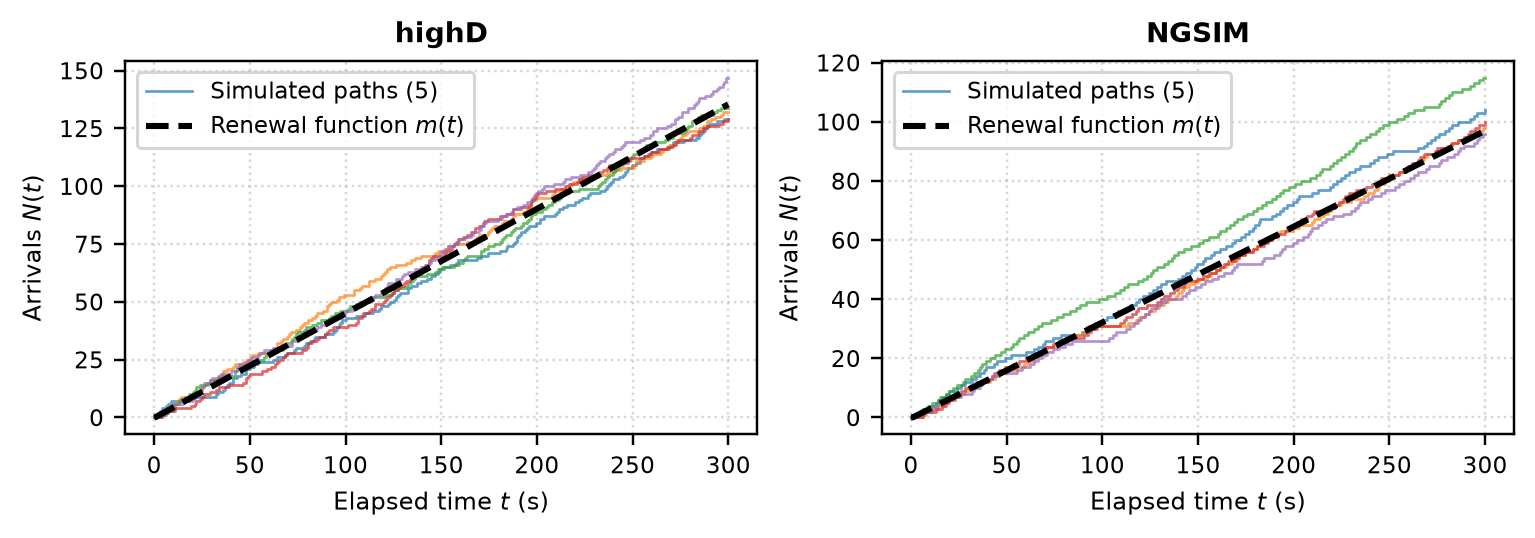
\includegraphics[width=\linewidth]{figures/fig_paths.png}
\caption{Five simulated sample paths of the arrival count $N(t)$ of the headway-driven renewal process (coloured) and the renewal function $m(t)$ (dashed).}\label{fig:paths}
\end{figure}

\begin{table}[H]
\centering\footnotesize
\setlength{\tabcolsep}{4pt}
\caption{Simulated renewal counts (2\,000 paths) against renewal theory, Eq.~\eqref{eq:renewal}. ``Var if Poisson'': variance of a Poisson process of the same rate $1/\mu$; errors are relative to theory.}
\label{tab:renewal}
\begin{tabular}{@{}llrrrrrrr@{}}
\toprule
Dataset & $t$ (s) & $\E N$ sim & $\E N$ theory & $\Var N$ sim & $\Var N$ theory & Var if Poisson & mean err & var err \\
\midrule
highD & 30 & 13.38 & 13.37 & 8.41 & 8.28 & 13.56 & 0.10\% & 1.6\% \\
 & 60 & 26.86 & 26.93 & 16.86 & 16.56 & 27.12 & 0.23\% & 1.8\% \\
 & 120 & 54.02 & 54.05 & 33.11 & 33.13 & 54.24 & 0.05\% & 0.0\% \\
 & 300 & 135.57 & 135.41 & 85.94 & 82.81 & 135.60 & 0.12\% & 3.8\% \\[0.3ex]
NGSIM & 30 & 9.47 & 9.45 & 4.12 & 4.43 & 9.73 & 0.18\% & 7.0\% \\
 & 60 & 19.16 & 19.18 & 8.50 & 8.86 & 19.45 & 0.12\% & 4.1\% \\
 & 120 & 38.72 & 38.63 & 17.20 & 17.71 & 38.90 & 0.24\% & 2.9\% \\
 & 300 & 96.95 & 96.98 & 46.37 & 44.28 & 97.26 & 0.04\% & 4.7\% 
\\
\bottomrule
\end{tabular}
\end{table}

The count variance is far below that of a Poisson process: at $t=300$~s it is 85.94 against 135.60 on highD and 46.37 against 97.26 on NGSIM (Table~\ref{tab:renewal}); the variance-to-mean ratio of Eq.~\eqref{eq:dispersion} is \hdCV{} (highD) and \ngCV{} (NGSIM), against 1 for Poisson.
Figure~\ref{fig:counts} shows the distribution of $N(60)$: its largest distance from the simulated distribution function is \hdKsNormal{} (highD) and \ngKsNormal{} (NGSIM) for the renewal-theory normal approximation, but \hdKsPoisson{} and \ngKsPoisson{} for a Poisson distribution of the same rate.
The renewal rates are \hdRate{} and \ngRate{} veh/s (\hdFlow{} and \ngFlow{} veh/h/lane). These are reciprocals of the mean headway of followers that have a leader, describe car-following states, and are not measured detector flows (Section~\ref{sec:valid}).

\begin{figure}[!tb]
\centering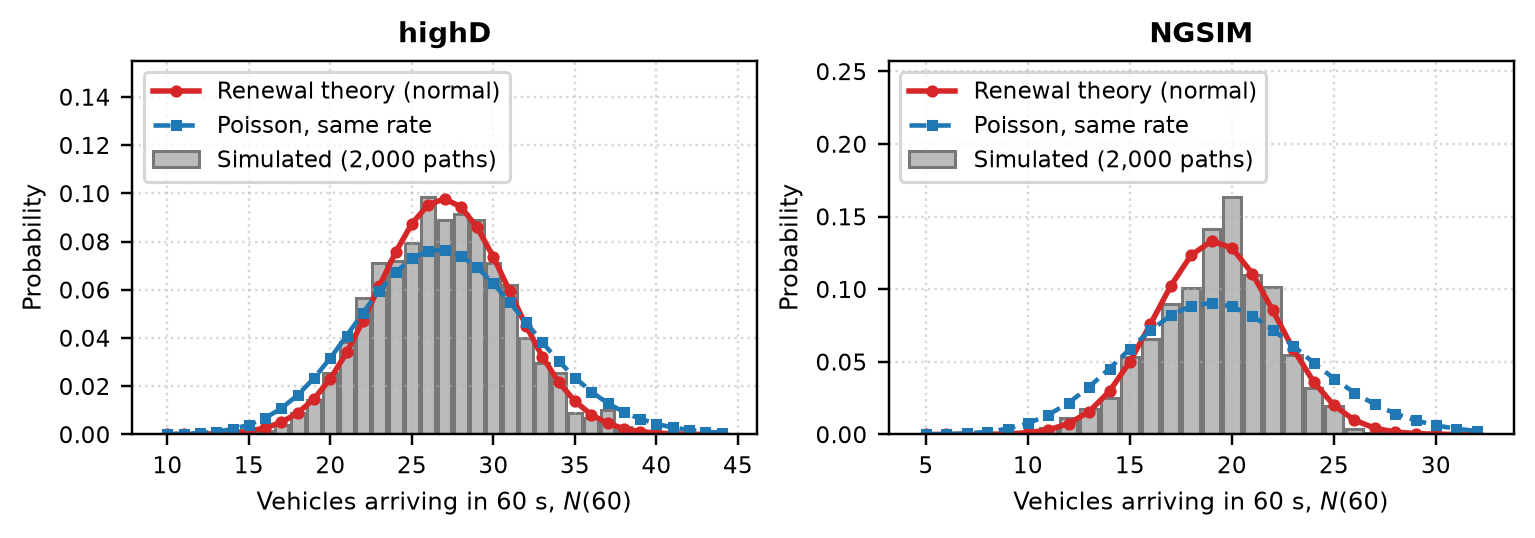
\includegraphics[width=\linewidth]{figures/fig_counts.png}
\caption{Distribution of the arrival count $N(60\text{ s})$: simulated renewal paths (bars), the renewal-theory normal approximation with continuity correction (red) and a Poisson process of the same rate (blue).}\label{fig:counts}
\end{figure}

\subsubsection{Regime Markov chain}\label{sec:markovres}
Table~\ref{tab:markov} gives the transition matrix, stationary distribution and mean recurrence times estimated from within-run transitions (\hdTrans{} on highD, \ngTrans{} on NGSIM), and Figure~\ref{fig:diagram} the chains as state-transition diagrams. Both chains are persistent, highD far more than NGSIM:
the model-implied expected sojourn $1/(1-p_{ii})$ is \hdSojC, \hdSojP{} and \hdSojF~s for close following, platoon and free flow on highD, and \ngSojC, \ngSojP{} and \ngSojF~s on NGSIM. Observed runs last only \hdRunLen~s (highD) and \ngRunLen~s (NGSIM) on average because a vehicle is observed only while it crosses the field of view and has a leader, so these sojourns are censored by the observation window and are model-implied expectations, not observed durations.
The regimes differ strongly between datasets: highD spends \hdPiC{} of the time in close following, \hdPiP{} in platoon and \hdPiF{} in free flow, whereas on NGSIM platoon dominates (\ngPiP), close following is rare (\ngPiC) and free flow accounts for \ngPiF. A highD trajectory returns to close following on average every \hdRecC{} s, an NGSIM trajectory only every \ngRecC{} s.
Figure~\ref{fig:stateprob} shows $\pi(n)=\pi(0)P^n$ from close following: the NGSIM chain is within total-variation distance \ngMixTVTwenty{} of its stationary law after 20~s, whereas the more persistent highD chain is at \hdMixTVTwenty{} after 20~s and \hdMixTVSixty{} after 60~s, much longer than its mean observed run.

\begin{table}[H]
\centering\small
\caption{Estimated transition matrix $P$ (rows: current regime, columns: next regime; one-second steps), stationary distribution $\pi$ and mean recurrence times $1/\pi_i$ (s).}
\label{tab:markov}
\begin{tabular}{@{}llrrrrr@{}}
\toprule
Dataset & From & $\to$ Close & $\to$ Platoon & $\to$ Free & $\pi_i$ & $1/\pi_i$ \\
\midrule
highD & Close following & 0.970 & 0.028 & 0.002 & 0.454 & 2.20 \\
 & Stable platoon & 0.028 & 0.961 & 0.011 & 0.435 & 2.30 \\
 & Free flow & 0.013 & 0.039 & 0.948 & 0.111 & 9.03 \\[0.3ex]
NGSIM & Close following & 0.746 & 0.245 & 0.009 & 0.096 & 10.42 \\
 & Stable platoon & 0.032 & 0.920 & 0.048 & 0.730 & 1.37 \\
 & Free flow & 0.004 & 0.202 & 0.794 & 0.174 & 5.75 
\\
\bottomrule
\end{tabular}
\end{table}

\begin{figure}[!tb]
\centering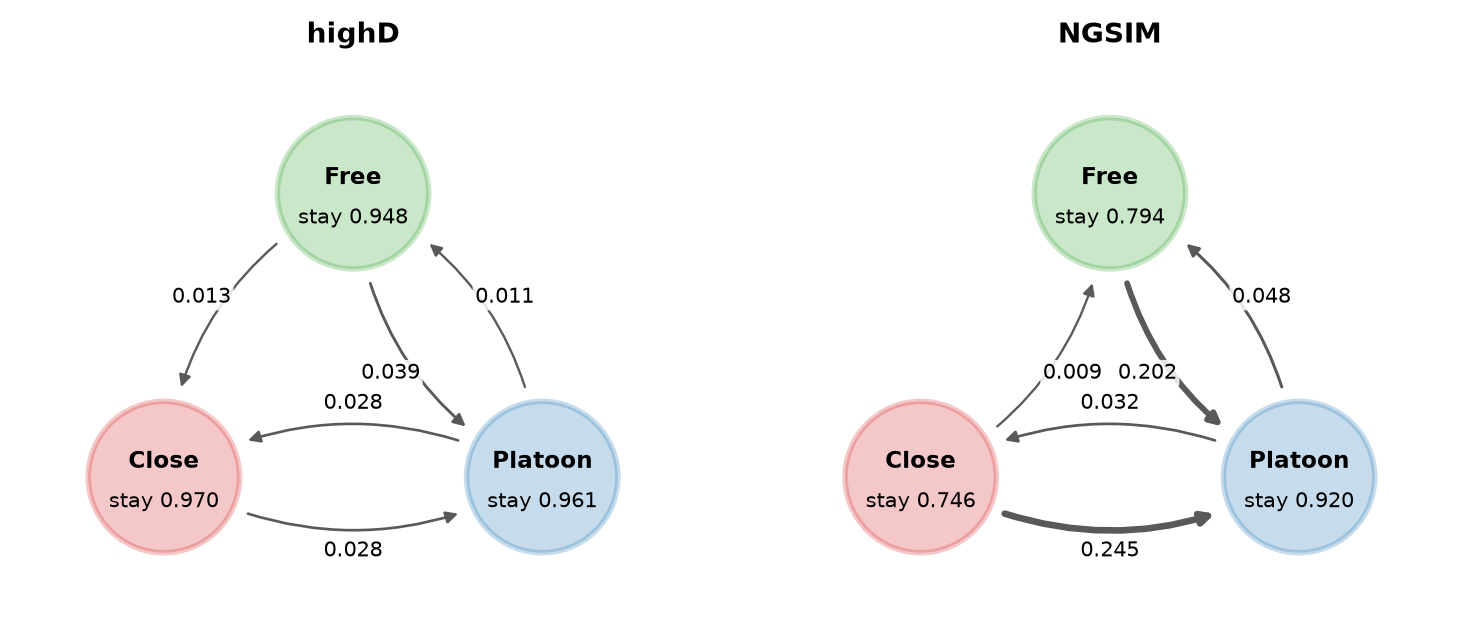
\includegraphics[width=\linewidth]{figures/fig_diagram.png}
\caption{State-transition diagrams of the regime Markov chains. Arrow labels are one-second transition probabilities $p_{ij}$, ``stay'' is $p_{ii}$, and arrow width grows with probability (transitions below 0.005 omitted).}\label{fig:diagram}
\end{figure}

\begin{figure}[!tb]
\centering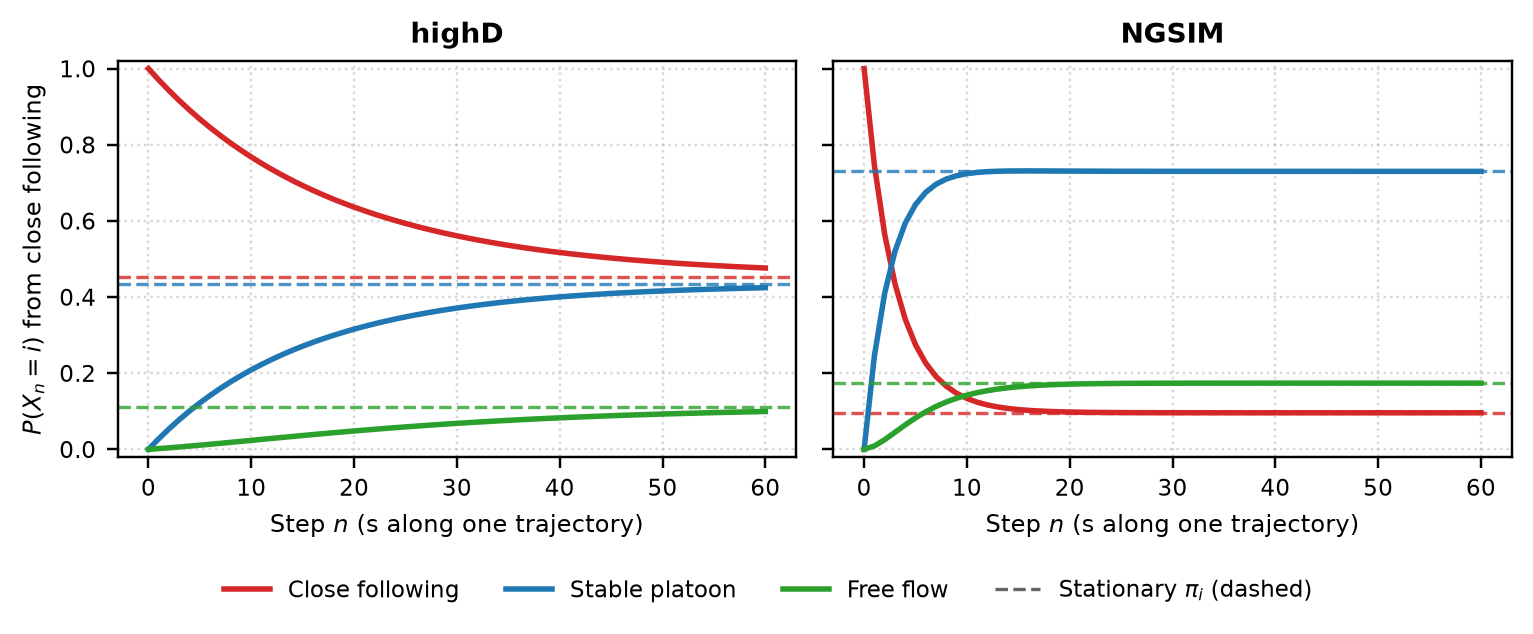
\includegraphics[width=\linewidth]{figures/fig_stateprob.png}
\caption{Transient regime probabilities $\pi(n)=\pi(0)P^n$ started from close following, with the stationary probabilities (dashed).}\label{fig:stateprob}
\end{figure}

\subsection{Real data results}\label{sec:real}
\subsubsection{Parameter estimates}
Table~\ref{tab:params} lists the posterior means of the seven distributions under the corrected (truncated) likelihood, the paper's likelihood, and as published~\cite{leungbootnak}. For the proposed distribution, highD gives $a=\hdA$~s (95\% credible interval [\hdALo, \hdAHi]; published 0.936) and $b=\hdB$ ([\hdBLo, \hdBHi]; published 0.540), i.e.\ $\kappa=\hdKappa$~s$^{-1}$;
NGSIM gives $a=\ngA$~s ([\ngALo, \ngAHi]; published 2.277), $b=\ngB$ ([\ngBLo, \ngBHi]; published 0.481) and $\kappa=\ngKappa$~s$^{-1}$ (Figure~\ref{fig:post}). The highD estimates are close to the published ones, the NGSIM estimates less so, as expected from the different NGSIM sample.
The two likelihoods agree for the proposed distribution and for the shifted-exponential rate $\lambda$ on both datasets, but differ for the other baselines on highD (Weibull shape 1.020 corrected against 1.450 with the paper likelihood; corrected gamma shape 1.117, near the exponential value 1).
The credible intervals are narrow because the multinomial likelihood treats samples as independent; they understate the true uncertainty since successive headways of a follower are strongly dependent (Section~\ref{sec:indep}).

\begin{table}[H]
\centering\footnotesize
\setlength{\tabcolsep}{4pt}
\caption{Posterior-mean parameters (names as in Table~\ref{tab:dists}) under the corrected (truncated) likelihood, the paper's likelihood, and as published~\cite{leungbootnak}. Under the truncated likelihood the shifted-exponential $\gamma$ is not identified (posterior = prior). The corrected NGSIM shifted log-normal $\gamma$ lies at its upper bound $\alpha=0.5$~s.}
\label{tab:params}
\begin{tabular}{@{}llrrrrrr@{}}
\toprule
 & & \multicolumn{3}{c}{highD} & \multicolumn{3}{c}{NGSIM} \\
\cmidrule(lr){3-5}\cmidrule(lr){6-8}
Distribution & Param. & Corrected & Paper lik. & Published & Corrected & Paper lik. & Published \\
\midrule
Proposed & $a$ & 0.954 & 0.954 & 0.936 & 2.336 & 2.336 & 2.277 \\
 & $b$ & 0.540 & 0.540 & 0.540 & 0.524 & 0.524 & 0.481 \\[0.3ex]
Shifted Log-normal & $\mu$ & 0.462 & 0.179 & 0.233 & 0.748 & 0.748 & 0.683 \\
 & $\sigma$ & 0.755 & 0.921 & 0.899 & 0.614 & 0.614 & 0.594 \\
 & $\gamma$ & \textminus{}0.001 & 0.438 & 0.377 & 0.500 & 0.500 & 0.528 \\[0.3ex]
Weibull & $\alpha$ & 1.020 & 1.450 & 1.481 & 1.533 & 1.678 & 1.744 \\
 & $\beta$ & 1.744 & 2.472 & 2.473 & 3.269 & 3.485 & 3.305 \\[0.3ex]
Log-logistic & $\alpha$ & 2.217 & 2.618 & 2.574 & 3.618 & 3.664 & 3.910 \\
 & $\beta$ & 1.565 & 1.717 & 1.719 & 2.613 & 2.617 & 2.515 \\[0.3ex]
Gamma & $\alpha$ & 1.117 & 2.304 & 2.335 & 3.479 & 3.693 & 4.175 \\
 & $\beta$ & 0.628 & 1.038 & 1.055 & 1.135 & 1.196 & 1.428 \\[0.3ex]
Burr & $\alpha$ & 1.464 & 3.777 & 3.199 & 4.916 & 4.896 & 5.237 \\
 & $\beta$ & 3.012 & 0.468 & 0.602 & 0.517 & 0.533 & 0.524 \\
 & $\lambda$ & 3.645 & 1.168 & 1.296 & 2.066 & 2.086 & 2.021 \\[0.3ex]
Shifted Exponential & $\lambda$ & 0.585 & 0.585 & 0.584 & 0.387 & 0.387 & 0.423 \\
 & $\gamma$ & \textit{not identified} & 0.500 & 0.500 & \textit{not identified} & 0.500 & 0.558
\\
\bottomrule
\end{tabular}
\end{table}

\subsubsection{Comparison of the seven distributions}\label{sec:gof}
Figure~\ref{fig:fits} overlays the fitted densities on the observed histograms, and Table~\ref{tab:gof} gives $D_{KL}$, $\Wvec$, $\Wtime$ and the one-sample KS statistic $D_1$ for the corrected fits, together with the paper-likelihood fits and the published values (where reported).

\begin{figure}[!tb]
\centering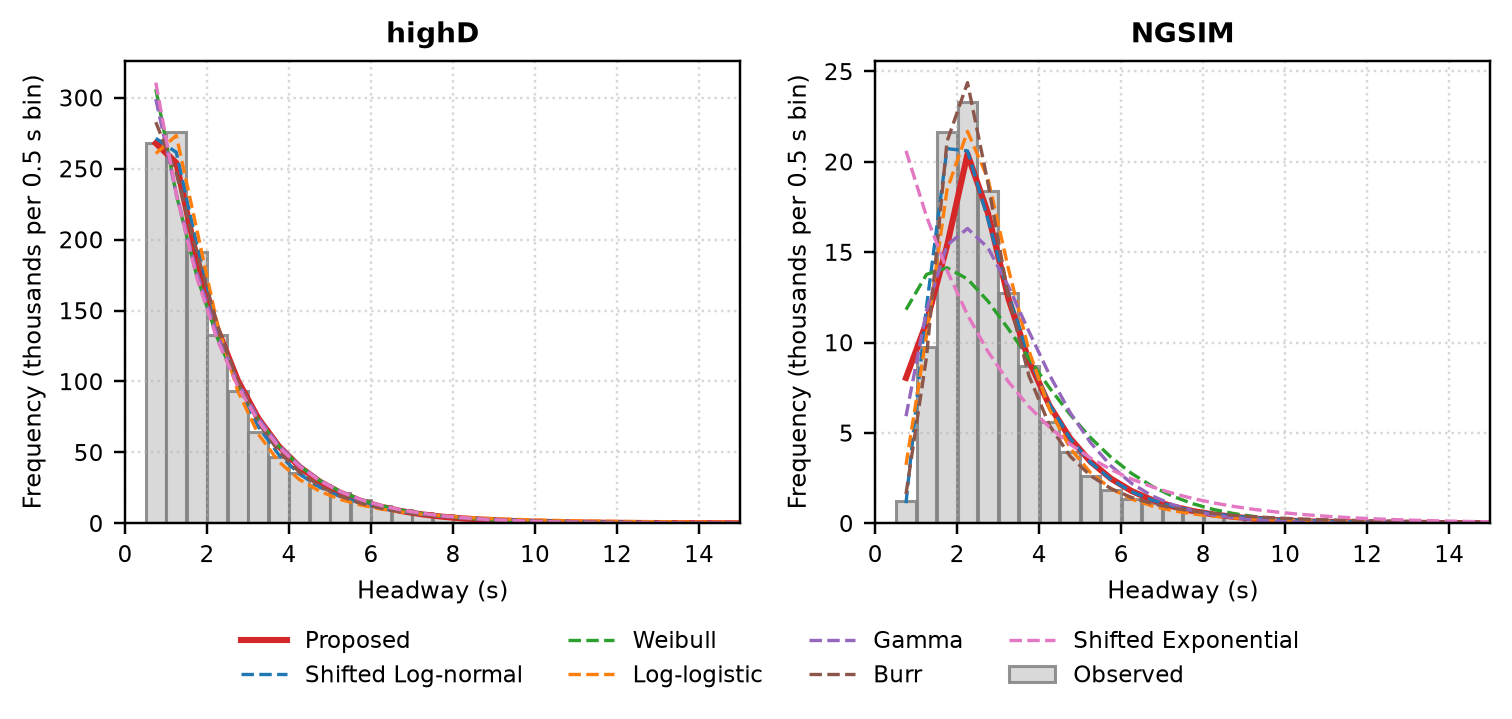
\includegraphics[width=\linewidth]{figures/fig_fits.png}
\caption{Observed headway histogram (bars) with the seven fitted distributions (corrected likelihood); curves show the expected count per 0.5~s bin of the window-conditioned model. The axis is cut at 15~s; the tail beyond is negligible.}\label{fig:fits}
\end{figure}

\begin{table}[H]
\centering\footnotesize
\setlength{\tabcolsep}{3pt}
\caption{Goodness of fit. $D_{KL}$ (unitless) and $\Wvec$ (unitless, Eq.~\eqref{eq:wvec}): corrected (Corr.) and paper (Paper) likelihood and published (Pub.) values from~\cite{leungbootnak}; $\Wtime$ (s, Eq.~\eqref{eq:wtime}; not reported in~\cite{leungbootnak}) and one-sample KS $D_1$: corrected fits. Lower is better; best of each of our columns in bold.}
\label{tab:gof}
\begin{tabular}{@{}lrrrrrrrr@{}}
\toprule
 & \multicolumn{3}{c}{$D_{KL}$} & \multicolumn{3}{c}{$\Wvec$} & $\Wtime$ & $D_1$ \\
\cmidrule(lr){2-4}\cmidrule(lr){5-7}
Distribution & Corr. & Paper & Pub. & Corr. & Paper & Pub. & Corr. & Corr. \\
\midrule
\multicolumn{9}{@{}l}{\textit{highD}} \\
Proposed & 0.0036 & \textbf{0.0036} & 0.0032 & 0.0012 & \textbf{0.0012} & 0.0011 & 0.072 & 0.025 \\
Shifted Log-normal & \textbf{0.0026} & 0.0063 & 0.0111 & \textbf{0.0008} & 0.0015 & 0.0016 & \textbf{0.048} & 0.013 \\
Weibull & 0.0079 & 0.0586 & 0.0534 & 0.0020 & 0.0058 & 0.0052 & 0.072 & 0.041 \\
Log-logistic & 0.0092 & 0.0229 & 0.0287 & 0.0013 & 0.0022 & 0.0026 & 0.130 & 0.016 \\
Gamma & 0.0075 & 0.0498 & 0.0454 & 0.0019 & 0.0050 & 0.0049 & 0.080 & 0.037 \\
Burr & 0.0043 & 0.0288 & 0.0332 & 0.0011 & 0.0033 & 0.0032 & 0.059 & 0.024 \\
Shifted Exponential & 0.0080 & 0.0080 & 0.0065 & 0.0021 & 0.0021 & 0.0018 & 0.064 & 0.044 \\
\midrule
\multicolumn{9}{@{}l}{\textit{NGSIM}} \\
Proposed & 0.0760 & 0.0760 & 0.0805 & 0.0043 & 0.0043 & 0.0040 & 0.225 & 0.076 \\
Shifted Log-normal & 0.0153 & 0.0153 & 0.0157 & 0.0022 & 0.0022 & 0.0021 & 0.155 & 0.030 \\
Weibull & 0.1871 & 0.1944 & 0.2098 & 0.0083 & 0.0090 & 0.0088 & 0.461 & 0.127 \\
Log-logistic & 0.0167 & 0.0168 & 0.0173 & 0.0021 & 0.0020 & 0.0020 & 0.156 & 0.026 \\
Gamma & 0.1142 & 0.1150 & 0.1182 & 0.0064 & 0.0063 & 0.0173 & 0.351 & 0.086 \\
Burr & \textbf{0.0015} & \textbf{0.0016} & 0.0027 & \textbf{0.0008} & \textbf{0.0009} & 0.0011 & \textbf{0.031} & 0.010 \\
Shifted Exponential & 0.2713 & 0.2713 & 0.3024 & 0.0050 & 0.0050 & 0.0047 & 0.645 & 0.228
\\
\bottomrule
\end{tabular}
\end{table}

\textbf{highD.} With the paper's likelihood the proposed distribution has the smallest $D_{KL}$ (\hdKLPropPaper) and $\Wvec$, as published; the shifted log-normal (0.0063) and shifted exponential (0.0080) follow. With the corrected likelihood the shifted log-normal is best by all three measures ($D_{KL}$ \hdKLSLN, $\Wtime$ \hdWtimeBestVal~s) and the proposed distribution is second by $D_{KL}$ (\hdKLProp), third by $\Wvec$ and fourth by $\Wtime$ (\hdWtimeProp~s).
The baselines improve markedly while the proposed distribution does not change: the $D_{KL}$ of the Weibull falls from 0.0586 to 0.0079, of the gamma from 0.0498 to 0.0075, of the Burr from 0.0288 to \hdKLBurr{} and of the log-logistic from 0.0229 to \hdKLLLog{} (factors of 2.4--7.4 for the five affected baselines). The published conclusion that the proposed distribution is best on highD thus holds under the published likelihood but not once the likelihood is conditioned on the window.
The reason is that the paper likelihood treats each baseline on its natural support, so $\sum_kp_k<1$ and mass below 0.5~s is penalised, which cannot happen to the proposed density (defined on $[\alpha,\infty)$); it also fits one distribution and evaluates another. The proposed distribution remains competitive, within the same order of divergence as the best with two parameters against three.
\textbf{NGSIM.} The Burr distribution is best by all three measures under both likelihoods ($D_{KL}$ \ngKLBurr, $\Wvec$ 0.0008, $\Wtime$ \ngWtimeBestVal~s), the shifted log-normal and log-logistic follow in $D_{KL}$ (\ngKLSLN{} and \ngKLLLog), and the proposed distribution is fourth by all three ($D_{KL}$ \ngKLProp, $\Wtime$ \ngWtimeProp~s). The shifted exponential is worst by $D_{KL}$ (0.2713) and $\Wtime$ (0.645~s), and the Weibull by $\Wvec$ (0.0083).
The likelihood hardly matters here, because NGSIM headways are longer and the baselines put little mass below 0.5~s (largest $D_{KL}$ change: Weibull, 0.1944 to 0.1871).
The two Wasserstein readings agree on the winner but not on lower ranks: on highD the log-logistic is fourth by $\Wvec$ (0.0013) but last by $\Wtime$ (0.130~s), illustrating that sorted-probability form is blind to the location of a mismatch.

\textbf{Hypothesis tests.} The chi-square test rejects every distribution on both datasets ($p<10^{-48}$; below $10^{-300}$ for 13 of the 14 fits). The two-sample KS test gives its smallest statistic for the corrected Burr distribution on NGSIM ($D=0.011$) but its $p$-value ($\approx7\times10^{-4}$) is also below 0.05.
With $10^5$--$10^6$ observations small departures are significant, so these tests do not discriminate, and $D$, $D_{KL}$ and the Wasserstein distances are more informative. The published study reports the same chi-square result but KS $p$-values near 1, which is not reproduced (its KS sample sizes are not stated); our $p$-values treat 1\,Hz samples as independent, which they are not.

\subsubsection{highD against NGSIM}\label{sec:disc}
The proposed distribution suits highD better than NGSIM, and the fitted curves suggest why: its density falls at the same rate on both sides of the mode. On highD the mode ($\hdA$~s) is only about 0.45~s above $\alpha$, so the left branch is short and the symmetry costs little;
on NGSIM the mode is at \ngA~s, the left branch spans about 1.8~s, the histogram rises faster to the mode than it decays after it, and a symmetric density with $\kappa=\ngKappa$~s$^{-1}$ overestimates the shortest headways (Figure~\ref{fig:fits}). The Burr, shifted log-normal and log-logistic distributions can represent this asymmetry (Burr shape $\alpha=\ngBurrAlpha$ on NGSIM: a peaked density with a heavy right tail).
This explanation is read from the fitted curves and the metrics and has not been tested with an asymmetric variant of the proposed density. In traffic terms, highD headways decay from a short mode near 0.95~s, whereas NGSIM has a distinct mode near 2.3~s with fewer very short headways than a symmetric law implies.

\subsection{Model validation}\label{sec:valid}
\subsubsection{MCMC convergence}\label{sec:conv}
All 28 fits ($7$ distributions $\times$ 2 datasets $\times$ 2 likelihoods) have $\hat R\le\ngRhatMaxPaper$ (Table~\ref{tab:diag}); the smallest ESS in the corrected runs is \hdEssMin{} (highD) and \ngEssMin{} (NGSIM) from 10\,000 retained draws, and acceptance rates are \ngAccMin--\ngAccMax\%, close to the optimum of about 23\%.
An earlier run of the paper likelihood with a random walk directly in $(\lambda,\gamma)$ gave $\hat R=4.92$ for the highD shifted exponential. This distribution alone has a binned log-likelihood \emph{linear} in $\gamma$ (it contains $N\lambda\gamma$), increasing until $\gamma$ reaches its upper limit $t_{\min}$, so the posterior of $\gamma$ is pressed against that limit with scale of order $1/(N\lambda)\sim10^{-6}$~s, a ridge ill-suited to a random walk with learned covariance.
Sampling $v=\log(t_{\min}-\gamma)$ removes the boundary: the rerun gives $\hat R=\hdRhatMaxPaper$ with posterior means $\lambda=\hdShExpLambdaPaper$ and $\gamma=\hdShExpGammaPaper$~s ($=t_{\min}$, as predicted), and a regression test checks $\hat R<1.05$ on a highD-sized sample. The value 4.92 belongs to the earlier sampler and is not a result of this paper; the diagnosis is inferred from the likelihood and supported by the success of the reparametrisation, not proved by it.

\begin{table}[H]
\centering\footnotesize
\setlength{\tabcolsep}{3pt}
\caption{MCMC convergence: largest split $\hat R$ over the parameters under the corrected (Trunc.) and paper likelihood, smallest effective sample size (ESS) and mean acceptance rate (Acc.) of the corrected run; two chains with 5\,000 post-warmup draws each.}
\label{tab:diag}
\begin{tabular}{@{}lrrrrrrrr@{}}
\toprule
 & \multicolumn{4}{c}{highD} & \multicolumn{4}{c}{NGSIM} \\
\cmidrule(lr){2-5}\cmidrule(lr){6-9}
Distribution & $\hat R$ Trunc. & $\hat R$ Paper & ESS & Acc. & $\hat R$ Trunc. & $\hat R$ Paper & ESS & Acc. \\
\midrule
Proposed & 1.001 & 1.001 & 1{,}231 & 25.6\% & 1.004 & 1.004 & 1{,}249 & 26.5\% \\
Shifted Log-normal & 1.002 & 1.003 & 951 & 21.0\% & 1.005 & 1.003 & 437 & 19.1\% \\
Weibull & 1.003 & 1.001 & 1{,}242 & 25.0\% & 1.002 & 1.002 & 1{,}181 & 25.0\% \\
Log-logistic & 1.004 & 1.002 & 1{,}286 & 25.2\% & 1.003 & 1.001 & 1{,}233 & 25.2\% \\
Gamma & 1.001 & 1.001 & 1{,}066 & 24.3\% & 1.003 & 1.002 & 1{,}282 & 25.7\% \\
Burr & 1.001 & 1.000 & 845 & 22.4\% & 1.002 & 1.006 & 936 & 22.5\% \\
Shifted Exponential & 1.002 & 1.005 & 609 & 22.3\% & 1.004 & 1.004 & 539 & 21.4\% 
\\
\bottomrule
\end{tabular}
\end{table}

\begin{figure}[!tb]
\centering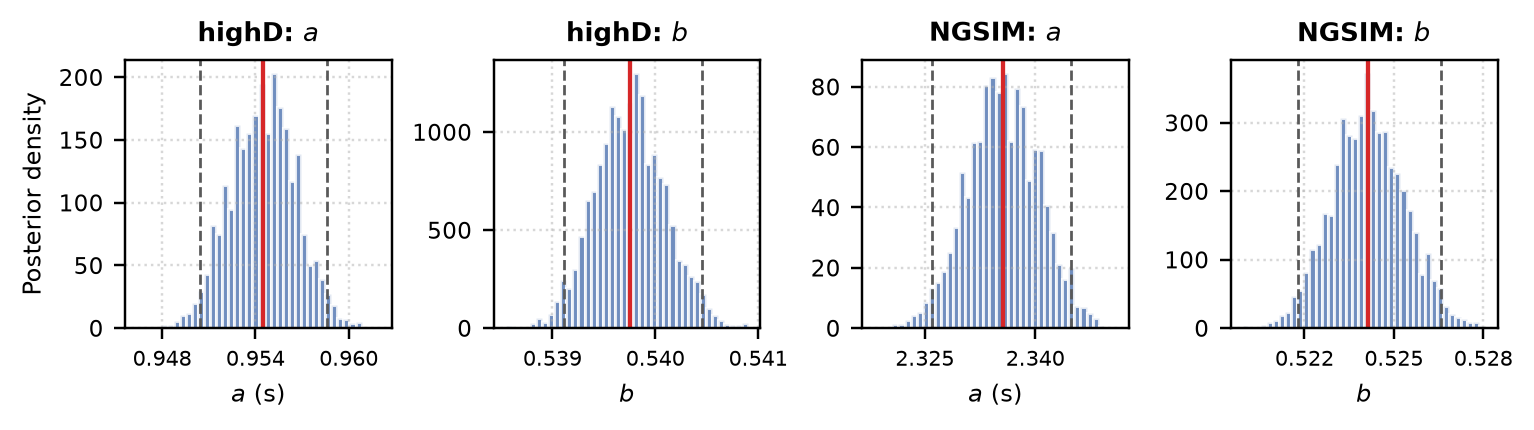
\includegraphics[width=\linewidth]{figures/fig_posterior.png}
\caption{Posterior distributions of the parameters $a$ (s) and $b$ of the proposed distribution (corrected likelihood): mean (red) and 95\% credible interval (dashed).}\label{fig:post}
\end{figure}

\subsubsection{Independence, autocorrelation and detector inter-arrival times}\label{sec:indep}
The renewal model assumes independent headways. The autocorrelation of one follower's one-second headways, computed only within runs (Table~\ref{tab:autocorr}), is \hdLagOne{} at lag 1 and \hdLagFive{} at lag 5 on highD (95\% white-noise band $\pm\hdBand$) and \ngLagOne{} and \ngLagFive{} on NGSIM:
successive headways of a follower are strongly dependent, as a driver's gap changes gradually. The 1\,Hz sample therefore cannot be treated as i.i.d., and the renewal simulation, which resamples independently, models the headway \emph{distribution} and not its temporal structure. This does not by itself show that detector inter-arrival times are dependent.

\begin{table}[H]
\centering\small
\caption{Autocorrelation at lags 1--5 of one-second headways within runs (Headways; lag in seconds) and of detector inter-arrival times (Detector gaps; lag in vehicles), with the half-width of the 95\% white-noise band.}
\label{tab:autocorr}
\begin{tabular}{@{}lrrrr@{}}
\toprule
 & \multicolumn{2}{c}{Headways (1\,Hz)} & \multicolumn{2}{c}{Detector gaps} \\
\cmidrule(lr){2-3}\cmidrule(lr){4-5}
Lag & highD & NGSIM & highD & NGSIM \\
\midrule
1 & 0.906 & 0.727 & 0.031 & 0.125 \\
2 & 0.820 & 0.614 & \textminus{}0.009 & 0.091 \\
3 & 0.740 & 0.535 & 0.017 & 0.091 \\
4 & 0.667 & 0.473 & 0.000 & 0.013 \\
5 & 0.601 & 0.426 & 0.008 & 0.034 \\
\midrule
95\% band $\pm$ & 0.0019 & 0.0058 & 0.0060 & 0.0434 
\\
\bottomrule
\end{tabular}
\end{table}

Detector crossings reconstructed as in Section~\ref{sec:detmethod} give \hdDetN{} inter-arrival times from \hdDetUnits{} lane-recordings on highD (mean \hdDetMean~s, \hdDetFlow{} veh/h/lane) and \ngDetN{} times from 6 lanes in the first NGSIM period (mean \ngDetMean~s, \ngDetFlow{} veh/h/lane).
The headway-driven rates (\hdFlow{} and \ngFlow{} veh/h/lane) are therefore not detector flows: higher on highD and lower on NGSIM, being reciprocals of the mean headway of followers that have a leader, sampled once per second. Detector gaps are almost uncorrelated on highD (lag-1 \hdDetLagOne{}, band $\pm\hdDetBand$, about zero later; Table~\ref{tab:autocorr}),
so independence is a reasonable approximation for the \emph{detector} process there, in contrast with the 1\,Hz headways; on NGSIM lag 1 is \ngDetLagOne{} (band $\pm\ngDetBand$) and lag 2 is \ngDetLagTwo{}, a modest dependence consistent with platooning, from only \ngDetN{} gaps at one position.
Table~\ref{tab:detcounts} compares count dispersion with the renewal prediction and Poisson. On highD in one-minute windows ($\hdDetWindows$ windows, \hdDetSeries{} series, mean count \hdDetMeanCount) the observed ratio is \hdDetFanoObs, against \hdDetFanoRen{} predicted from the same gaps and 1 for Poisson, much closer to Poisson than to the headway-driven prediction (\hdCV).
The excess over the renewal value is consistent with flow drifting within a recording. On NGSIM the observed ratio is \ngDetFanoObs{} at 60~s, well below Poisson, in line with the headway-driven value (\ngCV) and against \ngDetFanoRen{} for the renewal process of the detector gaps, from only \ngDetWindows{} windows; the detector gaps have $\mathrm{CV}^2=\ngDetCV$, different from the headway sample (\ngCV).
The reconstruction thus supports an approximately independent arrival process on highD and a regular, sub-Poisson one on NGSIM, but contradicts the claim that the dispersion of the headway distribution (\hdCV{} on highD) describes the variability of arrival counts. Limits: one detector position, non-stationary short recordings, and a single 15-minute NGSIM period.

\begin{table}[H]
\centering\small
\caption{Index of dispersion (variance/mean) of vehicle counts in consecutive $w$-second windows at the virtual detector: observed, renewal prediction $\sigma_u^2/\mu_u^2$ from the same series' gaps, and Poisson. Mean count: vehicles per window per lane.}
\label{tab:detcounts}
\begin{tabular}{@{}llrrrrr@{}}
\toprule
Dataset & $w$ (s) & Windows & Mean count & Observed & Renewal & Poisson \\
\midrule
highD & 30 & 10{,}986 & 9.8 & 0.94 & 0.77 & 1 \\
 & 60 & 5{,}383 & 19.5 & 0.96 & 0.77 & 1 \\
 & 120 & 2{,}493 & 39.5 & 0.97 & 0.76 & 1 \\[0.3ex]
NGSIM & 30 & 176 & 11.3 & 0.41 & 0.29 & 1 \\
 & 60 & 86 & 22.6 & 0.52 & 0.29 & 1 \\
 & 120 & 42 & 45.1 & 0.64 & 0.29 & 1 
\\
\bottomrule
\end{tabular}
\end{table}

\subsubsection{Markov-chain validation}
Table~\ref{tab:markovval} validates the chain on within-run regime sequences. The stationary distribution of $\hat P$ lies within total-variation distance \hdStatTV{} (highD) and \ngStatTV{} (NGSIM) of the observed regime fractions, consistent with within-run counting omitting the last sample of each run from the row totals; a long simulated path reproduces $\pi$ and re-estimates $P$ to within 0.0013 and 0.0064 (a check of the code).
\emph{Chapman--Kolmogorov:} the largest error of the empirical $n$-step matrix against $P^n$ is \hdCKtwo{} at $n=2$ and \hdCKfive{} at $n=5$ on highD, but \ngCKtwo{} and \ngCKfive{} on NGSIM. \emph{First against second order:} the likelihood-ratio test rejects the first-order chain on both datasets ($G^2=\hdSecondGsq$ and $\ngSecondGsq$, 12 d.f.), unavoidable with this many transitions, so the effect size matters: the mean total-variation distance between $P(\cdot\mid i,j)$ and $P(\cdot\mid j)$ is
\hdSecondTV{} on highD (negligible) and \ngSecondTV{} on NGSIM (small but real). The first-order chain therefore describes highD regimes adequately at short horizons and NGSIM regimes less well, where a semi-Markov or second-order model would be the natural extension.

\begin{table}[H]
\centering\small
\caption{Validation of the first-order regime Markov chain on within-run sequences. TV: total-variation distance; $G^2$: likelihood-ratio statistic of first against second order (both $p<10^{-200}$).}
\label{tab:markovval}
\begin{tabular}{@{}lrr@{}}
\toprule
Quantity & highD & NGSIM \\
\midrule
Chapman--Kolmogorov max error, $n=2$ & 0.006 & 0.092 \\
Chapman--Kolmogorov max error, $n=5$ & 0.055 & 0.226 \\
Stationary $\pi$ vs observed regime fractions (TV) & 0.0144 & 0.0084 \\
Simulated chain: occupation vs $\pi$ (TV) & 0.0123 & 0.0039 \\
Simulated chain: max error of re-estimated $P$ & 0.0013 & 0.0064 \\
Second-order test $G^2$ (12 d.f.) & 1046.4 & 4291.5 \\
Second-order effect size (mean TV) & 0.0014 & 0.0400
\\
\bottomrule
\end{tabular}
\end{table}

\subsubsection{Comparison with the published results}\label{sec:published}
With the paper's likelihood, our $D_{KL}$ differs from the published values by at most \hdKLMaxDiffPaper{} on highD (\hdKLMaxDiffPaperName) and \ngKLMaxDiffPaper{} on NGSIM (\ngKLMaxDiffPaperName), and $\Wvec$ by at most \hdWvecMaxDiffPaper{} (\hdWvecMaxDiffPaperName) and \ngWvecMaxDiffPaper{} (\ngWvecMaxDiffPaperName; the other six differ by 0.0003 or less).
The published $\Wvec$ for the gamma distribution on NGSIM (0.0173) is inconsistent with its own KL ranking, where the gamma has a lower divergence than the Weibull but twice the distance. The NGSIM ranking by $D_{KL}$ is identical to the published one. On highD only the second and third places differ (shifted exponential and shifted log-normal swap; published 0.0065 and 0.0111, ours 0.0080 and 0.0063).
Differences are largest for the badly fitting NGSIM baselines, which are sensitive to the exact sample, and the published NGSIM sample could not be reproduced (source and probably lane and time selection differ). Parameters agree closely on highD for the proposed distribution ($a=0.954$ against 0.936, $b$ identical) and less for the shifted log-normal and Burr, which are weakly identified under the paper likelihood.
The qualitative conclusions of~\cite{leungbootnak} are reproduced under the paper's likelihood (proposed best on highD, Burr best on NGSIM); the first is lost under the conditioned likelihood. The published KS $p$-values are not reproduced.

\subsection{Discussion}\label{sec:overall}
\textbf{Traffic regimes.} The datasets are in different states. highD is dominated by short headways and persistent regimes (close following \hdPiC{} and platoon \hdPiP{} of the time, with an expected close-following sojourn of \hdSojC~s), the normal state of an uninterrupted highway lane. NGSIM I-80 is dominated by platoon-range headways with few very short ones and less persistent regimes; the typical follower keeps two to three seconds.

\textbf{Arrivals: regular or nearly Poisson?} Followers' headways imply counts far less variable than Poisson, as car following suppresses both very short and very long gaps. Detector counts qualify this: they are sub-Poisson on NGSIM but close to Poisson on highD at the minute scale, presumably because gaps between vehicles at a point vary strongly between lanes and moments.
For queueing and signal-timing applications, a Poisson model is a reasonable description of highD-type uninterrupted flow at the minute scale but overstates variability in the I-80 sample, and the regularity should be taken from detector gaps, not followers' headways.

\textbf{Which distribution?} No distribution is best everywhere: Burr wins on NGSIM, the shifted log-normal wins on highD under the conditioned likelihood and the proposed distribution wins on highD under the paper's likelihood, so the lesson is the dependence of the ranking on dataset and fitting method. The proposed distribution offers two interpretable parameters (mode and decay rate), a closed-form distribution function and an easily sampled posterior, at the cost of a symmetry constraint that matters when the mode is far from the lower threshold.

\textbf{What the results do not show.} Since the goodness-of-fit tests reject every model, the results show relative, not absolute, adequacy; agreement of simulated counts with renewal theory verifies the simulation, not the independence assumption, which the 1\,Hz data contradict; and posterior uncertainty is conditional on independent samples and is optimistic.

%================================================================================================
\section{Limitations and Future Work}\label{sec:limits}
\textbf{Limitations.}
\begin{itemize}
  \item \emph{Likelihood.} The binned multinomial likelihood treats strongly autocorrelated 1\,Hz samples as independent (lag-1 \hdLagOne{} on highD), so credible intervals and KS $p$-values are too narrow; binning also discards within-bin information.
  \item \emph{Reproduction.} The published NGSIM sample is not reproduced (the first period was chosen by inference from the published parameters), nor are the published KS $p$-values and the gamma $\Wvec$ on NGSIM. Eq.~17 of~\cite{leungbootnak} is ambiguous, and $\Wvec$ and $\Wtime$ rank models differently.
  \item \emph{Renewal and Markov models.} The headway-driven process uses time headways, not detector inter-arrivals, and removes serial dependence by resampling; the detector validation uses one position per recording and, for NGSIM, one 15-minute period (\ngDetN{} gaps). Regime thresholds (1.5 s, 4 s) are modelling choices, sojourns are censored by the observation window, and the first-order assumption fails on NGSIM.
  \item \emph{Scope.} One seed, two human-driven datasets pooled over lanes, vehicle types and speeds, no covariates; the mixed human--automated datasets of the original study are not included.
\end{itemize}
\textbf{Future work} (proposals, not implemented): (i)~replace the independent binned likelihood by a model with serial dependence (for example a hidden or semi-Markov model with the regimes as states) and measure how much the posterior widens; (ii)~give the proposed density different decay rates on its two sides and test whether this restores its competitiveness on NGSIM;
(iii)~fit the seven distributions to detector inter-arrival times at several positions and relate them to flow; (iv)~make the distribution depend on speed and vehicle type, add the mixed human--automated datasets, and compare with composite tracking/free models~\cite{cowan1975}.

%================================================================================================
\section{Conclusion}\label{sec:conclusion}
Headways on two highway datasets were modelled with seven MCMC-fitted distributions, a renewal arrival process and a three-regime Markov chain. With the published likelihood the proposed distribution $f(t\mid a,b)\propto b^{|t-a|}$ is the best of seven on highD by $D_{KL}$ (\hdKLPropPaper) and fourth on NGSIM (\ngKLProp), where Burr is best (\ngKLBurr), reproducing the qualitative findings of~\cite{leungbootnak} to within \hdKLMaxDiffPaper{} and \ngKLMaxDiffPaper{} in $D_{KL}$.
Conditioning the likelihood on the $[0.5,25]$~s window, which the published method does not do, makes the shifted log-normal best on highD (\hdKLSLN) with the proposed distribution second (\hdKLProp): the published highD advantage comes partly from a likelihood that penalises distributions with mass below 0.5~s. All 28 posteriors converge, the earlier non-convergence of the highD shifted exponential being removed by reparametrising its threshold.

Simulated arrivals from the headways are far more regular than Poisson (variance-to-mean \hdCV{} and \ngCV) and agree with renewal theory, which verifies the simulation but not the model: against detector counts reconstructed from the trajectories, highD one-minute counts are nearly Poisson (\hdDetFanoObs) while NGSIM counts are sub-Poisson (\ngDetFanoObs), and although one-second headways of a follower are strongly autocorrelated (lag-1 \hdLagOne{} on highD), detector inter-arrival times are nearly independent on highD.
The stationary regime distributions are \hdPiC/\hdPiP/\hdPiF{} (close/platoon/free) on highD and \ngPiC/\ngPiP/\ngPiF{} on NGSIM, with the first-order chain adequate for highD at short horizons and less so for NGSIM.
The practical conclusions are that rankings of headway distributions depend on the likelihood used, that a headway distribution does not by itself determine the variability of arrival counts, and that stochastic models must be validated against data and not only against their own theory.

%================================================================================================
\bibliographystyle{unsrtnat}
\bibliography{references}

\appendix
\Needspace{16\baselineskip}
% Generated by final_report/make_code_excerpts.py from the repository source.
\section{Code Excerpts}\label{app:code}

\lstinputlisting[caption={Proposed headway distribution: normalised density and closed-form distribution function, Eqs.~\eqref{eq:density}--\eqref{eq:norm} (\texttt{headway/distributions.py}; docstrings omitted).},label={lst:dist}]{code/proposed_distribution.py}

\lstinputlisting[caption={Adaptive random-walk Metropolis--Hastings sampler: proposal, acceptance rule of Eq.~\eqref{eq:accept} and warmup-only adaptation (\texttt{headway/mcmc.py}; initialisation, covariance re-estimation and output handling omitted).},label={lst:mh}]{code/metropolis_sampler.py}

\lstinputlisting[caption={Simulation of the renewal counting process $N(t)$ from i.i.d.\ resampled headways (\texttt{headway/validation.py}).},label={lst:renewal}]{code/renewal_simulation.py}

\lstinputlisting[caption={Estimation of the regime transition matrix from within-run pairs of consecutive samples only (\texttt{headway/stochastic\_process.py}).},label={lst:markov}]{code/markov_estimation.py}


\end{document}
